\documentclass{scrreprt}

\usepackage{aligned-overset}
\usepackage{amsmath}
\usepackage{amssymb}
\usepackage{bm}
\usepackage[shortlabels]{enumitem}
\usepackage{hyperref}
\usepackage[utf8]{inputenc}
\usepackage{listings}
\usepackage{multicol}
\usepackage{mathtools}
\usepackage{physics}
\usepackage{stmaryrd}
\usepackage{tabularx}
\usepackage{titling}
\usepackage{fancyhdr}
\usepackage{xfrac}
\usepackage{pgfplots}

\pgfplotsset{compat = newest}
\usetikzlibrary{intersections}
\usetikzlibrary{patterns}
\usetikzlibrary{positioning}
\usetikzlibrary{shapes.misc}
\usepgfplotslibrary{fillbetween}

\author{Karsten Lehmann}
\date{WiSe 2021/2022}
\title{Übungsblatt 07\\Algorithmen und Datenstrukturen}

\setlength{\headheight}{26pt}
\pagestyle{fancy}
\fancyhf{}
\lhead{\thetitle}
\rhead{\theauthor}
\lfoot{\thedate}
\rfoot{Seite \thepage}

\begin{document}
\paragraph{Aufgabe 1} Wenden Sie den Quicksort-Algorithmus auf die Folge
$4, 7, 6, 2, 9$ an.
Die Zahlen sollen aufsteigend sortiert werden.
Dokumentieren Sie den Rechenablauf, indem Sie
\begin{itemize}
\item das Pivot-Element jeder Teilfolge kennzeichnen und
\item die Teilfolgen und Stellung der Indizes $i, j$ jeweils
  \begin{itemize}
  \item unmittelbar vor und nach jedem Tausch von Elementen, sowie
  \item unmittelbar vor und nach jedem rekursiven Aufruf angeben.
  \end{itemize}
\end{itemize}

\subparagraph{Lsg.}
\begin{enumerate}[label={\arabic*. Schritt}]
\item
  \begin{tabular}{ccccc}
    & & $\substack{\makebox[0pt]{\tiny Pivot-Element} \\ \downarrow}$ \\
    \hline
    \multicolumn{1}{|c}{4} & \multicolumn{1}{|c}{7} & \multicolumn{1}{|c}{6} & \multicolumn{1}{|c}{2} & \multicolumn{1}{|c|}{9} \\
    \hline
    & $\substack{\uparrow \\ i}$ & & $\substack{\uparrow \\ j}$
  \end{tabular}

\item
  \begin{tabular}{ccccc}
    & & $\substack{\makebox[0pt]{\tiny Pivot-Element} \\ \downarrow}$ \\
    \hline
    \multicolumn{1}{|c}{4} & \multicolumn{1}{|c}{2} & \multicolumn{1}{|c}{6} & \multicolumn{1}{|c}{7} & \multicolumn{1}{|c|}{9} \\
    \hline
    & $\substack{\uparrow \\ i}$ & & $\substack{\uparrow \\ j}$
  \end{tabular}

\item
  \begin{minipage}[t]{.4\textwidth}
     \begin{tabular}{ccc}
       $\substack{\makebox[0pt]{\tiny Pivot-Element} \\ \downarrow}$ \\
       \hline
       \multicolumn{1}{|c}{4} & \multicolumn{1}{|c|}{2} \\
       \hline
       $\substack{\uparrow \\ i}$ & $\substack{\uparrow \\ j}$ \\
     \end{tabular}
  \end{minipage}
  \hfill
  \vrule
  \hfill
  \begin{minipage}[t]{.4\textwidth}
    \begin{tabular}{ccc}
      $\substack{\makebox[0pt]{\tiny Pivot-Element} \\ \downarrow}$ \\
      \hline
      \multicolumn{1}{|c}{7} & \multicolumn{1}{|c|}{9} \\
      \hline
      $\substack{\uparrow \\ i}$ & $\substack{\uparrow \\ j}$
    \end{tabular}
  \end{minipage}

\item
  \begin{minipage}[t]{.4\textwidth}
     \begin{tabular}{cc}
       $\substack{\makebox[0pt]{\tiny Pivot-Element} \\ \downarrow}$ \\
       \hline
       \multicolumn{1}{|c}{2} & \multicolumn{1}{|c|}{4}\\
       \hline
       $\substack{\uparrow \\ i}$ & $\substack{\uparrow \\ j}$ \\
     \end{tabular}
  \end{minipage}
  \hfill
  \vrule
  \hfill
  \begin{minipage}[t]{.4\textwidth}
    \begin{tabular}{cc}
      $\substack{\makebox[0pt]{\tiny Pivot-Element} \\ \downarrow}$ \\
      \hline
      \multicolumn{1}{|c}{7} & \multicolumn{1}{|c|}{9} \\
      \hline
      $\substack{\uparrow \\ i}$ & $\substack{\uparrow \\ j}$
    \end{tabular}
  \end{minipage}

\item
  \begin{tabular}{ccccc}
    & & $\substack{\makebox[0pt]{\tiny Pivot-Element} \\ \downarrow}$ \\
    \hline
    \multicolumn{1}{|c}{2} & \multicolumn{1}{|c}{4} & \multicolumn{1}{|c}{6} & \multicolumn{1}{|c}{7} & \multicolumn{1}{|c|}{9} \\
    \hline
    & $\substack{\uparrow \\ i}$ & & $\substack{\uparrow \\ j}$
  \end{tabular}
\end{enumerate}

\newpage
\paragraph{Aufgabe 2}
Wenden Sie den Heapsort-Algorithmus auf die Folge
$2, 0, 9, 3, 5, 8, 4, 1, 6, 7$ an.
Dokumentieren Sie dazu in der Phase 1 das schrittweise Herstellen der
Heap-Eigenschaft und dabei insbesondere die Veränderungen durch die Funktion
``sinkenlassen''.
Das Sinkenlassen in mehreren \emph{unabhängigen} Teilbäumen darf in einem
Schritt protokolliert werden.
In der Phase 2 brauchen Sie nur zwei Sortierschritte ausführen.
Ein Sortierschritt besteht aus einem Tausch- und einem Sinkenlassen-Schritt, die
jeweils einzeln zu notieren sind.

\subparagraph{Lsg.}
\begin{enumerate}[label={\arabic*. Schritt:}]
\item Das Feld wird als Binärbaum abgebildet:

  \begin{tikzpicture}
    \node[circle, draw, label={160:{0}}] (0) {2};
    \node[below left = 1 and 1.5 of 0, circle, draw, label={160:{1}}] (1) {0};
    \node[below right = 1 and 1.5 of 0, circle, draw, label={180:{2}}] (2) {9};
    \node[below left = of 1, circle, draw, label={160:{3}}] (3) {3};
    \node[below right = 1 and 0.3 of 1, circle, draw, label={160:{4}}] (4) {5};
    \node[below left = 1 and 0.3 of 2, circle, draw, label={160:{5}}] (5) {8};
    \node[below right = of 2, circle, draw, label={170:{6}}] (6) {4};
    \node[below left = of 3, circle, draw, label={160:{7}}] (7) {1};
    \node[below right = 1 and 0.3 of 3, circle, draw, label={160:{8}}] (8) {6};
    \node[below right = 1 and 0 of 4, circle, draw, label={160:{9}}] (9) {7};
    \draw (0) -- (1);
    \draw (0) -- (2);
    \draw (1) -- (3);
    \draw (1) -- (4);
    \draw (2) -- (5);
    \draw (2) -- (6);
    \draw (3) -- (7);
    \draw (3) -- (8);
    \draw (4) -- (9);
  \end{tikzpicture}

\item Zuerst wird die maximale Position, die noch einen Nachfolger hat bestimmt.
  In diesem Beispiel ist dies die Position 4.
  Falls die Position kleiner als einer ihrer Nachfolger ist, so wird sie mit dem
  größeren Nachfolger vertauscht.
  In diesem Beispiel wird also die 5 auf Position 4 mit der 7 auf Position 9
  vertauscht - das sogenannte ``Sinkenlassen''.

  \begin{tikzpicture}
    \node[circle, draw, label={160:{0}}] (0) {2};
    \node[below left = 1 and 1.5 of 0, circle, draw, label={160:{1}}] (1) {0};
    \node[below right = 1 and 1.5 of 0, circle, draw, label={180:{2}}] (2) {9};
    \node[below left = of 1, circle, draw, label={160:{3}}] (3) {3};
    \node[below right = 1 and 0.3 of 1, circle, draw, label={160:{4}}] (4) {7};
    \node[below left = 1 and 0.3 of 2, circle, draw, label={160:{5}}] (5) {8};
    \node[below right = of 2, circle, draw, label={170:{6}}] (6) {4};
    \node[below left = of 3, circle, draw, label={160:{7}}] (7) {1};
    \node[below right = 1 and 0.3 of 3, circle, draw, label={160:{8}}] (8) {6};
    \node[below right = 1 and 0 of 4, circle, draw, label={160:{9}}] (9) {5};
    \draw (0) -- (1);
    \draw (0) -- (2);
    \draw (1) -- (3);
    \draw (1) -- (4);
    \draw (2) -- (5);
    \draw (2) -- (6);
    \draw (3) -- (7);
    \draw (3) -- (8);
    \draw (4) -- (9);
    \draw[<->, red, thick] (4) to[bend left] (9);
  \end{tikzpicture}

\newpage
\item Das ``Sinkenlassen'' wird an der Position 3 wiederholt.

  \begin{tikzpicture}
    \node[circle, draw, label={160:{0}}] (0) {2};
    \node[below left = 1 and 1.5 of 0, circle, draw, label={160:{1}}] (1) {0};
    \node[below right = 1 and 1.5 of 0, circle, draw, label={180:{2}}] (2) {9};
    \node[below left = of 1, circle, draw, label={160:{3}}] (3) {6};
    \node[below right = 1 and 0.3 of 1, circle, draw, label={160:{4}}] (4) {7};
    \node[below left = 1 and 0.3 of 2, circle, draw, label={160:{5}}] (5) {8};
    \node[below right = of 2, circle, draw, label={170:{6}}] (6) {4};
    \node[below left = of 3, circle, draw, label={160:{7}}] (7) {1};
    \node[below right = 1 and 0.3 of 3, circle, draw, label={160:{8}}] (8) {3};
    \node[below right = 1 and 0 of 4, circle, draw, label={160:{9}}] (9) {5};
    \draw (0) -- (1);
    \draw (0) -- (2);
    \draw (1) -- (3);
    \draw (1) -- (4);
    \draw (2) -- (5);
    \draw (2) -- (6);
    \draw (3) -- (7);
    \draw (3) -- (8);
    \draw (4) -- (9);
    \draw[<->, red, thick] (3) to[bend left] (8);
  \end{tikzpicture}

\item Das ``Sinkenlassen'' wird an der Position 1 wiederholt.
  Da die 0 auf Position 4 nun kleiner als der Nachfolger 0 auf Position 9 ist,
  werden auch diese beiden Positionen noch einmal vertauscht.

  \begin{tikzpicture}
    \node[circle, draw, label={160:{0}}] (0) {2};
    \node[below left = 1 and 1.5 of 0, circle, draw, label={160:{1}}] (1) {7};
    \node[below right = 1 and 1.5 of 0, circle, draw, label={180:{2}}] (2) {9};
    \node[below left = of 1, circle, draw, label={160:{3}}] (3) {6};
    \node[below right = 1 and 0.3 of 1, circle, draw, label={160:{4}}] (4) {5};
    \node[below left = 1 and 0.3 of 2, circle, draw, label={160:{5}}] (5) {8};
    \node[below right = of 2, circle, draw, label={170:{6}}] (6) {4};
    \node[below left = of 3, circle, draw, label={160:{7}}] (7) {1};
    \node[below right = 1 and 0.3 of 3, circle, draw, label={160:{8}}] (8) {3};
    \node[below right = 1 and 0 of 4, circle, draw, label={160:{9}}] (9) {0};
    \draw (0) -- (1);
    \draw (0) -- (2);
    \draw (1) -- (3);
    \draw (1) -- (4);
    \draw (2) -- (5);
    \draw (2) -- (6);
    \draw (3) -- (7);
    \draw (3) -- (8);
    \draw (4) -- (9);
    \draw[<->, red, thick] (1) to[bend left] (4);
    \draw[<->, red, thick] (4) to[bend left] (9);
  \end{tikzpicture}

\item Das ``Sinkenlassen'' wird an der Position 0 wiederholt.
  Da die 2 auf Position 9 nun kleiner als der Nachfolger 8 auf Position 5 ist,
  werden auch diese beiden Positionen noch einmal vertauscht.

  \begin{tikzpicture}
    \node[circle, draw, label={160:{0}}] (0) {9};
    \node[below left = 1 and 1.5 of 0, circle, draw, label={160:{1}}] (1) {7};
    \node[below right = 1 and 1.5 of 0, circle, draw, label={180:{2}}] (2) {8};
    \node[below left = of 1, circle, draw, label={160:{3}}] (3) {6};
    \node[below right = 1 and 0.3 of 1, circle, draw, label={160:{4}}] (4) {5};
    \node[below left = 1 and 0.3 of 2, circle, draw, label={160:{5}}] (5) {2};
    \node[below right = of 2, circle, draw, label={170:{6}}] (6) {4};
    \node[below left = of 3, circle, draw, label={160:{7}}] (7) {1};
    \node[below right = 1 and 0.3 of 3, circle, draw, label={160:{8}}] (8) {3};
    \node[below right = 1 and 0 of 4, circle, draw, label={160:{9}}] (9) {0};
    \draw (0) -- (1);
    \draw (0) -- (2);
    \draw (1) -- (3);
    \draw (1) -- (4);
    \draw (2) -- (5);
    \draw (2) -- (6);
    \draw (3) -- (7);
    \draw (3) -- (8);
    \draw (4) -- (9);
    \draw[<->, red, thick] (0) to[bend left] (2);
    \draw[<->, red, thick] (2) to[bend left] (5);
  \end{tikzpicture}

\newpage
\item Der Binärbaum ist nun ein Heap und es beginnt die 2. Phase.
  Die größte Zahl (die 9 auf Position 0) wird mit der Zahl auf der letzten
  Position (der 0 auf Position 9) getauscht.
  Die Position 9 ist nun nicht mehr Teil des Binärbaums.

  \begin{tikzpicture}
    \node[circle, draw, label={160:{0}}] (0) {0};
    \node[below left = 1 and 1.5 of 0, circle, draw, label={160:{1}}] (1) {7};
    \node[below right = 1 and 1.5 of 0, circle, draw, label={180:{2}}] (2) {8};
    \node[below left = of 1, circle, draw, label={160:{3}}] (3) {6};
    \node[below right = 1 and 0.3 of 1, circle, draw, label={160:{4}}] (4) {5};
    \node[below left = 1 and 0.3 of 2, circle, draw, label={160:{5}}] (5) {2};
    \node[below right = of 2, circle, draw, label={170:{6}}] (6) {4};
    \node[below left = of 3, circle, draw, label={160:{7}}] (7) {1};
    \node[below right = 1 and 0.3 of 3, circle, draw, label={160:{8}}] (8) {3};
    \node[below right = 1 and 0 of 4, draw, label={160:{9}}, rectangle] (9) {9};
    \draw (0) -- (1);
    \draw (0) -- (2);
    \draw (1) -- (3);
    \draw (1) -- (4);
    \draw (2) -- (5);
    \draw (2) -- (6);
    \draw (3) -- (7);
    \draw (3) -- (8);
    \draw[<->, red, thick] (0) to[bend left] (9);
  \end{tikzpicture}

\item Durch ``Sinkenlassen'' der Position 0 wird wieder ein Heap hergestellt.

  \begin{tikzpicture}
    \node[circle, draw, label={160:{0}}] (0) {8};
    \node[below left = 1 and 1.5 of 0, circle, draw, label={160:{1}}] (1) {7};
    \node[below right = 1 and 1.5 of 0, circle, draw, label={180:{2}}] (2) {4};
    \node[below left = of 1, circle, draw, label={160:{3}}] (3) {6};
    \node[below right = 1 and 0.3 of 1, circle, draw, label={160:{4}}] (4) {5};
    \node[below left = 1 and 0.3 of 2, circle, draw, label={160:{5}}] (5) {2};
    \node[below right = of 2, circle, draw, label={170:{6}}] (6) {0};
    \node[below left = of 3, circle, draw, label={160:{7}}] (7) {1};
    \node[below right = 1 and 0.3 of 3, circle, draw, label={160:{8}}] (8) {3};
    \node[below right = 1 and 0 of 4, draw, label={160:{9}}, rectangle] (9) {9};
    \draw (0) -- (1);
    \draw (0) -- (2);
    \draw (1) -- (3);
    \draw (1) -- (4);
    \draw (2) -- (5);
    \draw (2) -- (6);
    \draw (3) -- (7);
    \draw (3) -- (8);
    \draw[<->, red, thick] (0) to[bend left] (2);
    \draw[<->, red, thick] (2) to[bend left] (6);
  \end{tikzpicture}

\item Die größte Zahl (in Position 0) wird wieder mit der letzten Position
  getauscht.

  \begin{tikzpicture}
    \node[circle, draw, label={160:{0}}] (0) {3};
    \node[below left = 1 and 1.5 of 0, circle, draw, label={160:{1}}] (1) {7};
    \node[below right = 1 and 1.5 of 0, circle, draw, label={180:{2}}] (2) {4};
    \node[below left = of 1, circle, draw, label={160:{3}}] (3) {6};
    \node[below right = 1 and 0.3 of 1, circle, draw, label={160:{4}}] (4) {5};
    \node[below left = 1 and 0.3 of 2, circle, draw, label={160:{5}}] (5) {2};
    \node[below right = of 2, circle, draw, label={170:{6}}] (6) {0};
    \node[below left = of 3, circle, draw, label={160:{7}}] (7) {1};
    \node[below right = 1 and 0.3 of 3, draw, label={160:{8}}, rectangle] (8) {8};
    \node[below right = 1 and 0 of 4, draw, label={160:{9}}, rectangle] (9) {9};
    \draw (0) -- (1);
    \draw (0) -- (2);
    \draw (1) -- (3);
    \draw (1) -- (4);
    \draw (2) -- (5);
    \draw (2) -- (6);
    \draw (3) -- (7);
    \draw[<->, red, thick] (0) to[out=-80,in=20] (8);
  \end{tikzpicture}

\newpage
\item Durch ``Sinkenlassen'' der Position 0 wird wieder ein Heap hergestellt.

  \begin{tikzpicture}
    \node[circle, draw, label={160:{0}}] (0) {7};
    \node[below left = 1 and 1.5 of 0, circle, draw, label={160:{1}}] (1) {6};
    \node[below right = 1 and 1.5 of 0, circle, draw, label={180:{2}}] (2) {4};
    \node[below left = of 1, circle, draw, label={160:{3}}] (3) {3};
    \node[below right = 1 and 0.3 of 1, circle, draw, label={160:{4}}] (4) {5};
    \node[below left = 1 and 0.3 of 2, circle, draw, label={160:{5}}] (5) {2};
    \node[below right = of 2, circle, draw, label={170:{6}}] (6) {0};
    \node[below left = of 3, circle, draw, label={160:{7}}] (7) {1};
    \node[below right = 1 and 0.3 of 3, draw, label={160:{8}}, rectangle] (8) {8};
    \node[below right = 1 and 0 of 4, draw, label={160:{9}}, rectangle] (9) {9};
    \draw (0) -- (1);
    \draw (0) -- (2);
    \draw (1) -- (3);
    \draw (1) -- (4);
    \draw (2) -- (5);
    \draw (2) -- (6);
    \draw (3) -- (7);
    \draw[<->, red, thick] (0) to[bend right] (1);
    \draw[<->, red, thick] (1) to[bend right] (3);
  \end{tikzpicture}

\item Die größte Zahl (in Position 0) wird wieder mit der letzten Position
  getauscht.

  \begin{tikzpicture}
    \node[circle, draw, label={160:{0}}] (0) {1};
    \node[below left = 1 and 1.5 of 0, circle, draw, label={160:{1}}] (1) {6};
    \node[below right = 1 and 1.5 of 0, circle, draw, label={180:{2}}] (2) {4};
    \node[below left = of 1, circle, draw, label={160:{3}}] (3) {3};
    \node[below right = 1 and 0.3 of 1, circle, draw, label={160:{4}}] (4) {5};
    \node[below left = 1 and 0.3 of 2, circle, draw, label={160:{5}}] (5) {2};
    \node[below right = of 2, circle, draw, label={170:{6}}] (6) {0};
    \node[below left = of 3, draw, label={160:{7}}, rectangle] (7) {7};
    \node[below right = 1 and 0.3 of 3, draw, label={160:{8}}, rectangle] (8) {8};
    \node[below right = 1 and 0 of 4, draw, label={160:{9}}, rectangle] (9) {9};
    \draw (0) -- (1);
    \draw (0) -- (2);
    \draw (1) -- (3);
    \draw (1) -- (4);
    \draw (2) -- (5);
    \draw (2) -- (6);
    \draw[<->, red, thick] (0) to[out=190, in=80] (7);
  \end{tikzpicture}

\item Durch ``Sinkenlassen'' der Position 0 wird wieder ein Heap hergestellt.

  \begin{tikzpicture}
    \node[circle, draw, label={160:{0}}] (0) {6};
    \node[below left = 1 and 1.5 of 0, circle, draw, label={160:{1}}] (1) {5};
    \node[below right = 1 and 1.5 of 0, circle, draw, label={180:{2}}] (2) {4};
    \node[below left = of 1, circle, draw, label={160:{3}}] (3) {3};
    \node[below right = 1 and 0.3 of 1, circle, draw, label={160:{4}}] (4) {1};
    \node[below left = 1 and 0.3 of 2, circle, draw, label={160:{5}}] (5) {2};
    \node[below right = of 2, circle, draw, label={170:{6}}] (6) {0};
    \node[below left = of 3, draw, label={160:{7}}, rectangle] (7) {7};
    \node[below right = 1 and 0.3 of 3, draw, label={160:{8}}, rectangle] (8) {8};
    \node[below right = 1 and 0 of 4, draw, label={160:{9}}, rectangle] (9) {9};
    \draw (0) -- (1);
    \draw (0) -- (2);
    \draw (1) -- (3);
    \draw (1) -- (4);
    \draw (2) -- (5);
    \draw (2) -- (6);
    \draw[<->, red, thick] (0) to[bend right] (1);
    \draw[<->, red, thick] (1) to[bend left] (4);
  \end{tikzpicture}

\newpage
\item Die größte Zahl (in Position 0) wird wieder mit der letzten Position
  getauscht.

  \begin{tikzpicture}
    \node[circle, draw, label={160:{0}}] (0) {0};
    \node[below left = 1 and 1.5 of 0, circle, draw, label={160:{1}}] (1) {5};
    \node[below right = 1 and 1.5 of 0, circle, draw, label={180:{2}}] (2) {4};
    \node[below left = of 1, circle, draw, label={160:{3}}] (3) {3};
    \node[below right = 1 and 0.3 of 1, circle, draw, label={160:{4}}] (4) {1};
    \node[below left = 1 and 0.3 of 2, circle, draw, label={160:{5}}] (5) {2};
    \node[below right = of 2, circle, draw, label={170:{6}}, rectangle] (6) {6};
    \node[below left = of 3, draw, label={160:{7}}, rectangle] (7) {7};
    \node[below right = 1 and 0.3 of 3, draw, label={160:{8}}, rectangle] (8) {8};
    \node[below right = 1 and 0 of 4, draw, label={160:{9}}, rectangle] (9) {9};
    \draw (0) -- (1);
    \draw (0) -- (2);
    \draw (1) -- (3);
    \draw (1) -- (4);
    \draw (2) -- (5);
    \draw[<->, red, thick] (0) to[bend left] (6);
  \end{tikzpicture}

\item Durch ``Sinkenlassen'' der Position 0 wird wieder ein Heap hergestellt.

  \begin{tikzpicture}
    \node[circle, draw, label={160:{0}}] (0) {5};
    \node[below left = 1 and 1.5 of 0, circle, draw, label={160:{1}}] (1) {3};
    \node[below right = 1 and 1.5 of 0, circle, draw, label={180:{2}}] (2) {4};
    \node[below left = of 1, circle, draw, label={160:{3}}] (3) {0};
    \node[below right = 1 and 0.3 of 1, circle, draw, label={160:{4}}] (4) {1};
    \node[below left = 1 and 0.3 of 2, circle, draw, label={160:{5}}] (5) {2};
    \node[below right = of 2, circle, draw, label={170:{6}}, rectangle] (6) {6};
    \node[below left = of 3, draw, label={160:{7}}, rectangle] (7) {7};
    \node[below right = 1 and 0.3 of 3, draw, label={160:{8}}, rectangle] (8) {8};
    \node[below right = 1 and 0 of 4, draw, label={160:{9}}, rectangle] (9) {9};
    \draw (0) -- (1);
    \draw (0) -- (2);
    \draw (1) -- (3);
    \draw (1) -- (4);
    \draw (2) -- (5);
    \draw[<->, red, thick] (0) to[bend right] (1);
    \draw[<->, red, thick] (1) to[bend right] (3);
  \end{tikzpicture}

\item Die größte Zahl (in Position 0) wird wieder mit der letzten Position
  getauscht.

  \begin{tikzpicture}
    \node[circle, draw, label={160:{0}}] (0) {2};
    \node[below left = 1 and 1.5 of 0, circle, draw, label={160:{1}}] (1) {3};
    \node[below right = 1 and 1.5 of 0, circle, draw, label={180:{2}}] (2) {4};
    \node[below left = of 1, circle, draw, label={160:{3}}] (3) {0};
    \node[below right = 1 and 0.3 of 1, circle, draw, label={160:{4}}] (4) {1};
    \node[below left = 1 and 0.3 of 2, draw, label={160:{5}}, rectangle] (5) {5};
    \node[below right = of 2, circle, draw, label={170:{6}}, rectangle] (6) {6};
    \node[below left = of 3, draw, label={160:{7}}, rectangle] (7) {7};
    \node[below right = 1 and 0.3 of 3, draw, label={160:{8}}, rectangle] (8) {8};
    \node[below right = 1 and 0 of 4, draw, label={160:{9}}, rectangle] (9) {9};
    \draw (0) -- (1);
    \draw (0) -- (2);
    \draw (1) -- (3);
    \draw (1) -- (4);
    \draw[<->, red, thick] (0) to[in=180, out=240] (5);
  \end{tikzpicture}

\newpage
\item Durch ``Sinkenlassen'' der Position 0 wird wieder ein Heap hergestellt.

  \begin{tikzpicture}
    \node[circle, draw, label={160:{0}}] (0) {4};
    \node[below left = 1 and 1.5 of 0, circle, draw, label={160:{1}}] (1) {3};
    \node[below right = 1 and 1.5 of 0, circle, draw, label={180:{2}}] (2) {2};
    \node[below left = of 1, circle, draw, label={160:{3}}] (3) {0};
    \node[below right = 1 and 0.3 of 1, circle, draw, label={160:{4}}] (4) {1};
    \node[below left = 1 and 0.3 of 2, draw, label={160:{5}}, rectangle] (5) {5};
    \node[below right = of 2, circle, draw, label={170:{6}}, rectangle] (6) {6};
    \node[below left = of 3, draw, label={160:{7}}, rectangle] (7) {7};
    \node[below right = 1 and 0.3 of 3, draw, label={160:{8}}, rectangle] (8) {8};
    \node[below right = 1 and 0 of 4, draw, label={160:{9}}, rectangle] (9) {9};
    \draw (0) -- (1);
    \draw (0) -- (2);
    \draw (1) -- (3);
    \draw (1) -- (4);
    \draw[<->, red, thick] (0) to[bend left] (2);
  \end{tikzpicture}

\item Die größte Zahl (in Position 0) wird wieder mit der letzten Position
  getauscht.

  \begin{tikzpicture}
    \node[circle, draw, label={160:{0}}] (0) {1};
    \node[below left = 1 and 1.5 of 0, circle, draw, label={160:{1}}] (1) {3};
    \node[below right = 1 and 1.5 of 0, circle, draw, label={180:{2}}] (2) {2};
    \node[below left = of 1, circle, draw, label={160:{3}}] (3) {0};
    \node[below right = 1 and 0.3 of 1, draw, label={160:{4}}, rectangle] (4) {4};
    \node[below left = 1 and 0.3 of 2, draw, label={160:{5}}, rectangle] (5) {5};
    \node[below right = of 2, circle, draw, label={170:{6}}, rectangle] (6) {6};
    \node[below left = of 3, draw, label={160:{7}}, rectangle] (7) {7};
    \node[below right = 1 and 0.3 of 3, draw, label={160:{8}}, rectangle] (8) {8};
    \node[below right = 1 and 0 of 4, draw, label={160:{9}}, rectangle] (9) {9};
    \draw (0) -- (1);
    \draw (0) -- (2);
    \draw (1) -- (3);
    \draw[<->, red, thick] (0) to[bend left] (4);
  \end{tikzpicture}

\item Durch ``Sinkenlassen'' der Position 0 wird wieder ein Heap hergestellt.

  \begin{tikzpicture}
    \node[circle, draw, label={160:{0}}] (0) {3};
    \node[below left = 1 and 1.5 of 0, circle, draw, label={160:{1}}] (1) {1};
    \node[below right = 1 and 1.5 of 0, circle, draw, label={180:{2}}] (2) {2};
    \node[below left = of 1, circle, draw, label={160:{3}}] (3) {0};
    \node[below right = 1 and 0.3 of 1, draw, label={160:{4}}, rectangle] (4) {4};
    \node[below left = 1 and 0.3 of 2, draw, label={160:{5}}, rectangle] (5) {5};
    \node[below right = of 2, circle, draw, label={170:{6}}, rectangle] (6) {6};
    \node[below left = of 3, draw, label={160:{7}}, rectangle] (7) {7};
    \node[below right = 1 and 0.3 of 3, draw, label={160:{8}}, rectangle] (8) {8};
    \node[below right = 1 and 0 of 4, draw, label={160:{9}}, rectangle] (9) {9};
    \draw (0) -- (1);
    \draw (0) -- (2);
    \draw (1) -- (3);
    \draw[<->, red, thick] (0) to[bend right] (1);
  \end{tikzpicture}

\newpage
\item Die größte Zahl (in Position 0) wird wieder mit der letzten Position
  getauscht.

  \begin{tikzpicture}
    \node[circle, draw, label={160:{0}}] (0) {0};
    \node[below left = 1 and 1.5 of 0, circle, draw, label={160:{1}}] (1) {1};
    \node[below right = 1 and 1.5 of 0, circle, draw, label={180:{2}}] (2) {2};
    \node[below left = of 1, draw, label={160:{3}}, rectangle] (3) {3};
    \node[below right = 1 and 0.3 of 1, draw, label={160:{4}}, rectangle] (4) {4};
    \node[below left = 1 and 0.3 of 2, draw, label={160:{5}}, rectangle] (5) {5};
    \node[below right = of 2, circle, draw, label={170:{6}}, rectangle] (6) {6};
    \node[below left = of 3, draw, label={160:{7}}, rectangle] (7) {7};
    \node[below right = 1 and 0.3 of 3, draw, label={160:{8}}, rectangle] (8) {8};
    \node[below right = 1 and 0 of 4, draw, label={160:{9}}, rectangle] (9) {9};
    \draw (0) -- (1);
    \draw (0) -- (2);
    \draw[<->, red, thick] (0) to[bend right] (3);
  \end{tikzpicture}

\item Durch ``Sinkenlassen'' der Position 0 wird wieder ein Heap hergestellt.

  \begin{tikzpicture}
    \node[circle, draw, label={160:{0}}] (0) {2};
    \node[below left = 1 and 1.5 of 0, circle, draw, label={160:{1}}] (1) {1};
    \node[below right = 1 and 1.5 of 0, circle, draw, label={180:{2}}] (2) {0};
    \node[below left = of 1, draw, label={160:{3}}, rectangle] (3) {3};
    \node[below right = 1 and 0.3 of 1, draw, label={160:{4}}, rectangle] (4) {4};
    \node[below left = 1 and 0.3 of 2, draw, label={160:{5}}, rectangle] (5) {5};
    \node[below right = of 2, circle, draw, label={170:{6}}, rectangle] (6) {6};
    \node[below left = of 3, draw, label={160:{7}}, rectangle] (7) {7};
    \node[below right = 1 and 0.3 of 3, draw, label={160:{8}}, rectangle] (8) {8};
    \node[below right = 1 and 0 of 4, draw, label={160:{9}}, rectangle] (9) {9};
    \draw (0) -- (1);
    \draw (0) -- (2);
    \draw[<->, red, thick] (0) to[bend left] (2);
  \end{tikzpicture}

\item Die größte Zahl (in Position 0) wird wieder mit der letzten Position
  getauscht.

  \begin{tikzpicture}
    \node[circle, draw, label={160:{0}}] (0) {0};
    \node[below left = 1 and 1.5 of 0, circle, draw, label={160:{1}}] (1) {1};
    \node[below right = 1 and 1.5 of 0, draw, label={180:{2}}, rectangle] (2) {2};
    \node[below left = of 1, draw, label={160:{3}}, rectangle] (3) {3};
    \node[below right = 1 and 0.3 of 1, draw, label={160:{4}}, rectangle] (4) {4};
    \node[below left = 1 and 0.3 of 2, draw, label={160:{5}}, rectangle] (5) {5};
    \node[below right = of 2, circle, draw, label={170:{6}}, rectangle] (6) {6};
    \node[below left = of 3, draw, label={160:{7}}, rectangle] (7) {7};
    \node[below right = 1 and 0.3 of 3, draw, label={160:{8}}, rectangle] (8) {8};
    \node[below right = 1 and 0 of 4, draw, label={160:{9}}, rectangle] (9) {9};
    \draw (0) -- (1);
    \draw[<->, red, thick] (0) to[bend left] (2);
  \end{tikzpicture}

\newpage
\item Durch ``Sinkenlassen'' der Position 0 wird wieder ein Heap hergestellt.

  \begin{tikzpicture}
    \node[circle, draw, label={160:{0}}] (0) {1};
    \node[below left = 1 and 1.5 of 0, circle, draw, label={160:{1}}] (1) {0};
    \node[below right = 1 and 1.5 of 0, draw, label={180:{2}}, rectangle] (2) {2};
    \node[below left = of 1, draw, label={160:{3}}, rectangle] (3) {3};
    \node[below right = 1 and 0.3 of 1, draw, label={160:{4}}, rectangle] (4) {4};
    \node[below left = 1 and 0.3 of 2, draw, label={160:{5}}, rectangle] (5) {5};
    \node[below right = of 2, circle, draw, label={170:{6}}, rectangle] (6) {6};
    \node[below left = of 3, draw, label={160:{7}}, rectangle] (7) {7};
    \node[below right = 1 and 0.3 of 3, draw, label={160:{8}}, rectangle] (8) {8};
    \node[below right = 1 and 0 of 4, draw, label={160:{9}}, rectangle] (9) {9};
    \draw (0) -- (1);
    \draw[<->, red, thick] (0) to[bend left] (1);
  \end{tikzpicture}

\item Die größte Zahl (in Position 0) wird wieder mit der letzten Position
  getauscht.

  \begin{tikzpicture}
    \node[draw, label={160:{0}}, rectangle] (0) {0};
    \node[below left = 1 and 1.5 of 0, draw, label={160:{1}}, rectangle] (1) {1};
    \node[below right = 1 and 1.5 of 0, draw, label={180:{2}}, rectangle] (2) {2};
    \node[below left = of 1, draw, label={160:{3}}, rectangle] (3) {3};
    \node[below right = 1 and 0.3 of 1, draw, label={160:{4}}, rectangle] (4) {4};
    \node[below left = 1 and 0.3 of 2, draw, label={160:{5}}, rectangle] (5) {5};
    \node[below right = of 2, circle, draw, label={170:{6}}, rectangle] (6) {6};
    \node[below left = of 3, draw, label={160:{7}}, rectangle] (7) {7};
    \node[below right = 1 and 0.3 of 3, draw, label={160:{8}}, rectangle] (8) {8};
    \node[below right = 1 and 0 of 4, draw, label={160:{9}}, rectangle] (9) {9};
    \draw[<->, red, thick] (0) to[bend left] (1);
  \end{tikzpicture}
\end{enumerate}
\end{document}